%*----------- SLIDE -------------------------------------------------------------
 %*----------- SLIDE (IMAGEM DO PROJETO) -------------------------------------------------------------
 \begin{frame}[t]{OPEN Manipulator Pro}
    \begin{figure}
        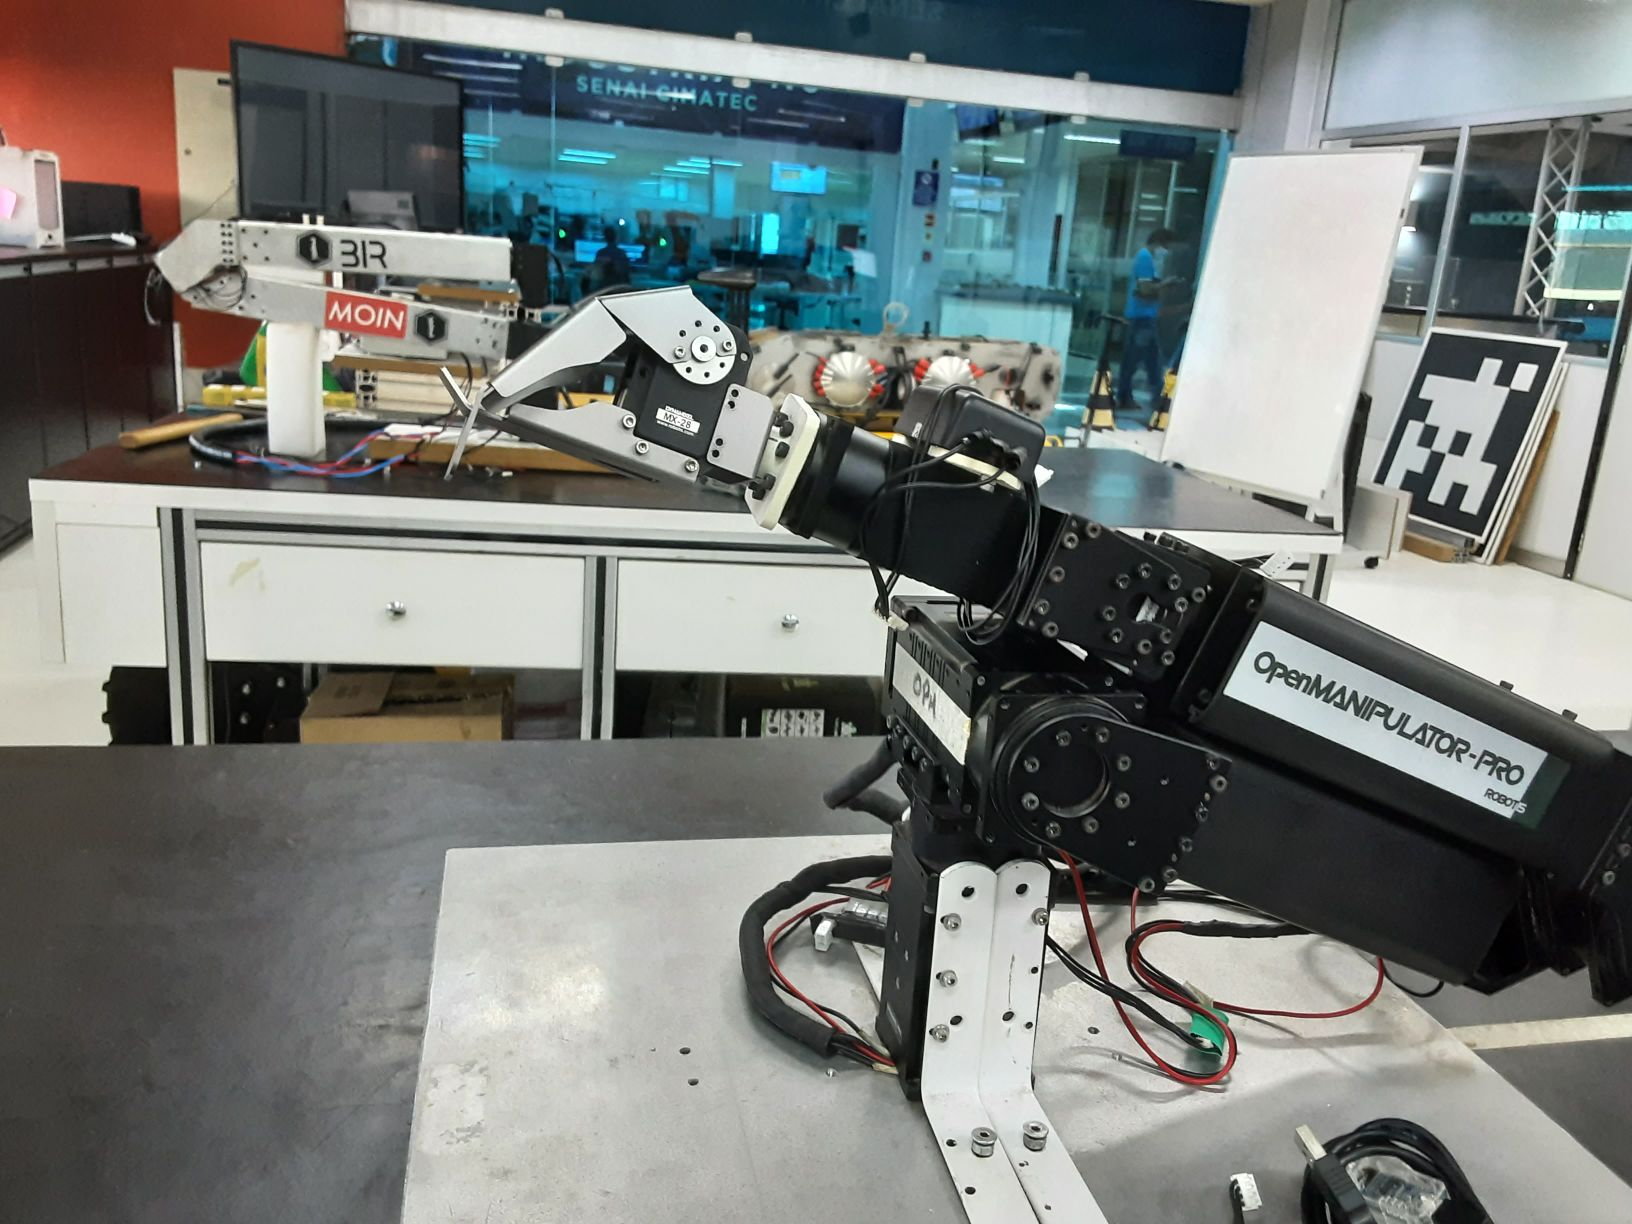
\includegraphics[width=0.60\textwidth]{manipulador.jpg}
        %\caption{.}
    \end{figure}
\end{frame}
 %*----------- SLIDE (IMAGEM DO PROJETO) -------------------------------------------------------------
 \begin{frame}[t]{Andamento do projeto}
    \begin{figure}
        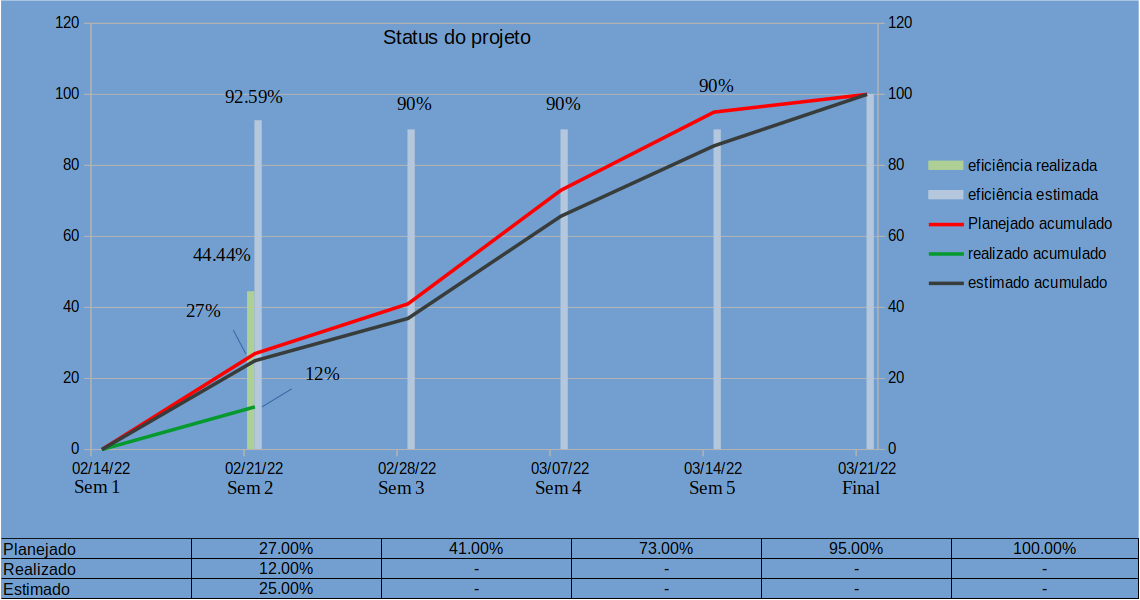
\includegraphics[width=0.85\textwidth]{planejamento-follow-up-16-02-2022.png}
        %\caption{.}
    \end{figure}
\end{frame}

%-------------------------------------------------------------
\begin{frame}[c]{Andamento do projeto}
    \begin{table}[ht!]
    \centering
        \caption{PERCENTUAL DE CONCLUSÃO}
        \begin{tabular}{|c|c|c|c|c|} \hline
            \textbf{Estado Anterior}&\textbf{Estado Atual}&\textbf{Eficiência}\\\hline
            0\% &12\% &44.44\% \\ \hline
        \end{tabular}
    \end{table}
    \begin{table}[ht!]
        %\centering
            \caption{ATIVIDADES REALIZADAS}
            \begin{tabular}{|c|c|c|c|} \hline
                \textbf{Atividade}&\textbf{Porcentagem}&\textbf{Atividade}&\textbf{Porcentagem}\\\hline
                Verificar documentações &60\% &   WBS        &80\% \\ \hline
                Customer Requirements   &0\%  &   PBS        &80  \% \\ \hline
                Arquitetura Geral       &50\% &   Simulação  &0\%  \\ \hline

            \end{tabular}
        \end{table}
%*----------- notes
    \note[item]{Notes can help you to remember important information. Turn on the notes option.}
\end{frame}
%-